
\chapter{Structure and Design}

\epigraph{In general, when modeling phenomena in science and
  engineering, we begin with simplified, incomplete models. As we
  examine things in greater detail, these simple models become
  inadequate and must be replaced by more refined
  models.}{\textit{Structure and Interpretation of Computer Programs,
    Section 1.1.5}\cite{sicp}}

\section{Structure of combox}

\begin{figure}[h]
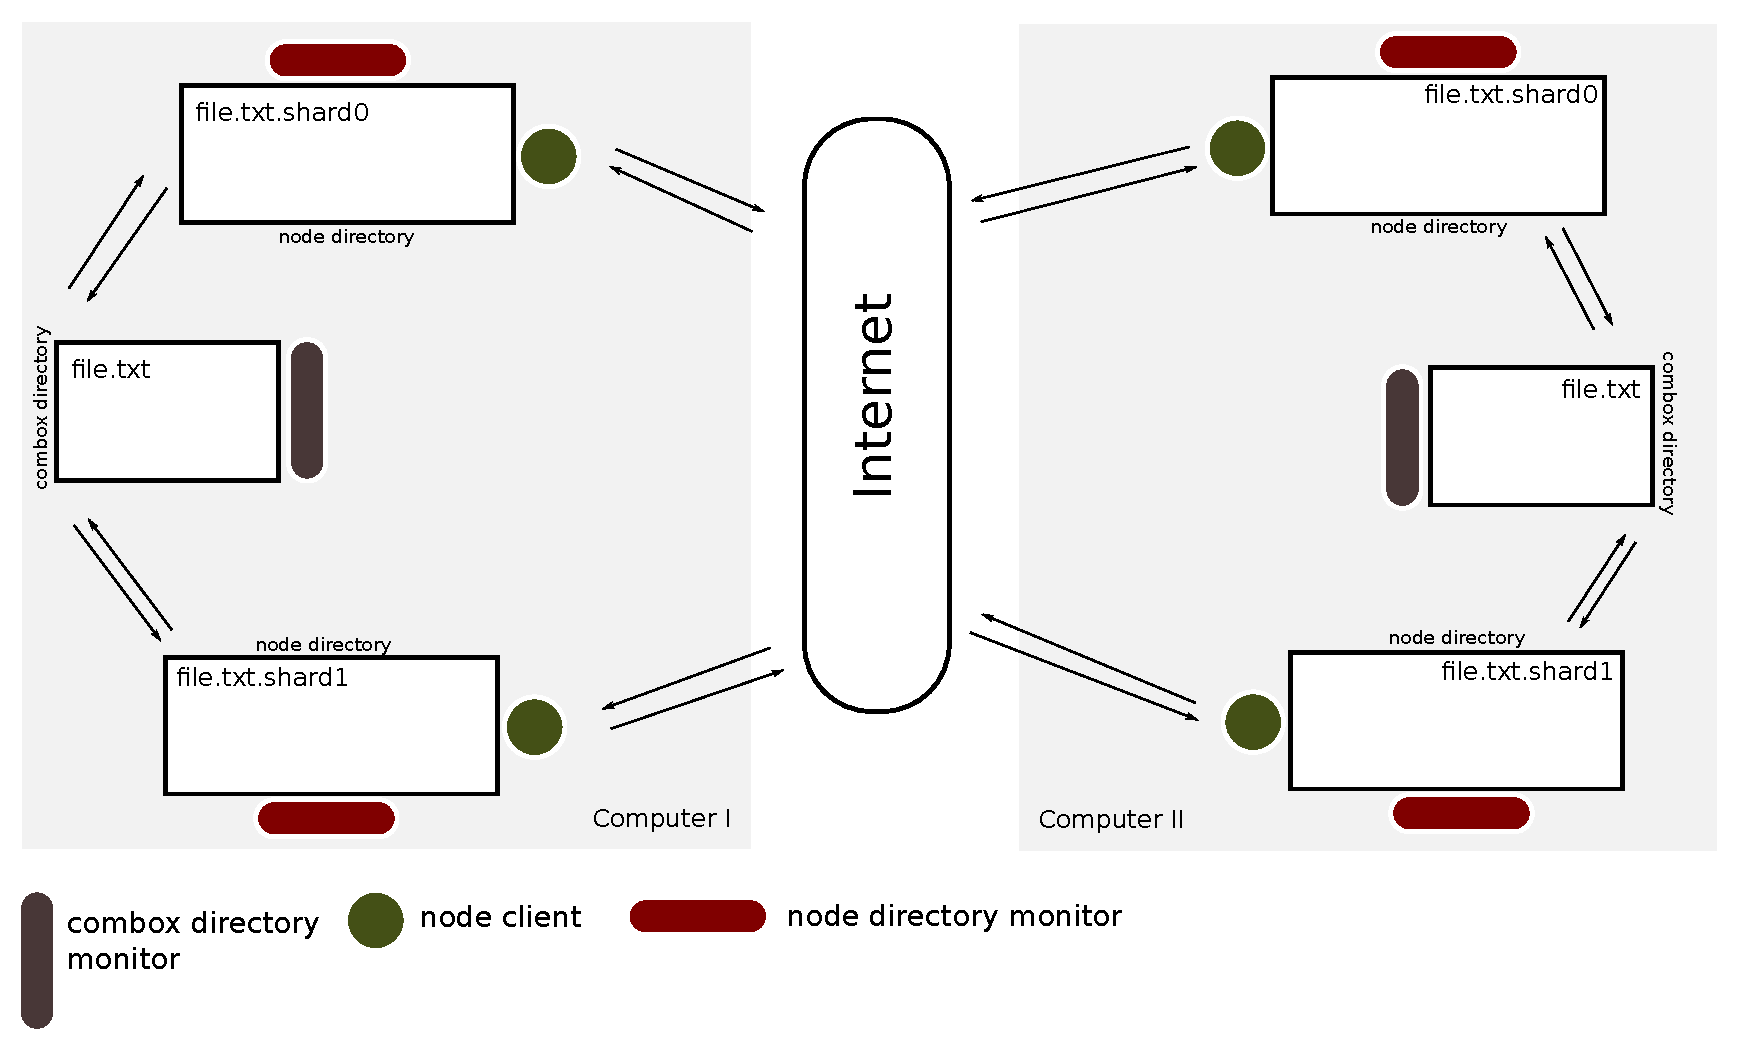
\includegraphics[scale=0.6]{4-combox-structure}
\caption{High level view of combox on two computers.}
\label{fig:4-combox-structure}
\end{figure}

\subsection{combox configuration}

\subsection{combox directory monitor}

\subsection{Node directory monitor}

\subsection{Database structure}

\section{combox modules overview}

combox is spread into modules that have functions and/or classes. As
of \verb+2016-02-04+ combox is considerably a small program:

\begin{verbatim}
$ wc -l combox/*.py
  144 combox/cbox.py
  178 combox/config.py
  241 combox/crypto.py
  891 combox/events.py
  541 combox/file.py
  454 combox/gui.py
    0 combox/__init__.py
   71 combox/log.py
  278 combox/silo.py
   29 combox/_version.py
 2827 total
\end{verbatim}

This section gives an overview of each of the combox modules with
extreme brevity:

\begin{description}
\item[combox.cbox] This module contains \verb+run_cb+ function runs
  combox; it creates an instance \verb+threading.Lock+ for database
  access and a shared \verb+threading.Lock+ for the
  \verb+combox.events.ComboxDirMonitor+ and
  \verb+combox.events.NodeDirMonitor+; it initializes an instance
  \verb+combox.events.ComboxDirMonitor+ that monitors the combox
  directory and an instance of \verb+combox.events.NodeDirMonitor+ for
  each node directory for monitoring the node directories. This
  modules also houses the \verb+main+ function that parses commandline
  arguments, starts combox configuration if needed or loads the combox
  configuration file to start running combox.
\item[combox.config] Accomodates two import functions --
  \verb+config_cb+ and \verb+get_nodedirs+. The \verb+config_cb+ is
  the combox configuration function that allows the user to configure
  combox; this function was designed in a such way that it was
  possible to use for both CLI and GUI methods of configuring
  combox. The \verb+get_nodedirs+ function returns, as a list, the
  paths of the node directories; this function use used in numerous
  places in other combox modules.
\item[combox.crypto] This has functions for encrypting and decrypting
  data; encrypting and decrypting shards (\verb+encrypt_shards+ and
  \verb+decrypt_shards+); a function for splitting a file into shards,
  encrypting those shards and spreading them across node directories
  (\verb+split_and_encrypt+); a function for decrypting the shards
  from the node directories, reconstructing the file from the
  decrypted shards and put the file back to the combox directory
  (\verb+decrypt_and_glue+). Functions \verb+split_and_encrypt+ and
  \verb+decrypt_and_glue+ are the two functions that that are
  extensively used by the \verb+combox.events+ module; all other
  functions in this module are pretty much helper functions are
  \verb+split_and_encrypt+ and \verb+decrypt_and_glue+ functions and
  are not used by other modules.
\item[combox.events] This module took the most time to write and test
  and it is the most complex module in combox at the time of writing
  this report. It contains just two classes -- \verb+ComboxDirMonitor+
  and \verb+NodeDirMonitor+. The \verb+ComboxDirMonitor+ inherits the
  \verb+watchdog.events.LoggingEventHandler+ and is responsible for
  monitoring for changes in the combox directory and doing the right
  thing when change happens in the combox directory. The
  \verb+NodeDirMonitor+ also inherits
  \verb+watchdog.events.LoggingEventHandler+ and similarly responsible
  for monitoring a node directory and doing the right thing when a
  change happens in the node directory; subjectively,
  \verb+NodeDirMonitor+ is slightly more complex than the
  \verb+ComboxDirMonitor+.
\item[combox.file] This is the second largest module in combox. It
  contains utility functions for reading, writing, moving
  files/directiores, hashing files, splitting a file into shards, glue
  shards into a file, manipulating directories inside combox and node
  directories.
\item[combox.gui]
\item[combox.log]
\item[combox.silo]
\item[combox.\_version]

\end{description}

\section{Language choice and DRY}

\section{Operating system compatibility}

\section{combox as a python package}

\section{With the benefit of hindsight}